\newpage

\section*{Soluzioni}

\subsection*{Punto 1}

Lo stesso codice pu\`o essere organizzato in diversi
modi. Nell'implementazione fornita, un unico \emph{file} contiene la
definizione di tutti i tipi e le funzioni utilizzate da
\cpp{main()}.

\lstset{basicstyle=\scriptsize\sf}
\lstinputlisting[caption=Soluzione dell'esercitazione 3:
organizzazione monolitica del codice.]{es/1/bn.monolithic.cpp}
\lstset{basicstyle=\sf}

A partire da questo codice � possibile ricavare la struttura
analizzata nella terza esercitazione: un \emph{file}
\texttt{rootfinding.hpp}
che contiene nomi e variabili generali; un \emph{file} \texttt{zerofun.hpp}
che contiene le \emph{dichiarazioni} delle procedure implementate per
la ricerca di zeri di una funzione analitica e un \emph{file}
\texttt{zerofun.cpp} che ne contiene le definizioni.

La figura \ref{fig:dep_graph} illustra l'organizzazione del codice in due
\textbf{unit\`a di compilazione}. Le immagini sono state generate
da \texttt{Doxygen} sulla base della documentazione del codice che
risolve l'esercitazione 3, grazie alle
funzionalit\`a offerte dal software \texttt{GraphViz}
(\texttt{http://www.graphviz.org/}).

\begin{figure}
\subfigure[\texttt{bn.cpp}]{
\includegraphics{./bn_8cpp__incl.eps}
}
\subfigure[\texttt{zerofun.cpp}]{
\includegraphics{./zerofun_8cpp__incl.eps}
}
\caption{Grafico delle dipendenze per le unit\`a di compilazione}
\label{fig:dep_graph}
\end{figure}

Si noti che l'organizzazione in unit\`a di compilazione
aiuta a suddividere il codice in \emph{moduli} semantici o funzionali,
migliorando la leggibilit\`a e l'efficienza: la scelta tra
un'organizzazione modulare o monolitica del codice risponde
essenzialmente a criteri di stile di programmazione.

Si noti tuttavia che, in una unit\`a di compilazione, il ruolo dei
\emph{source files} (\texttt{*.cpp}) \`e nettamente distinto da quello
degli \emph{header files} (\texttt{*.hpp}). Ad
esempio, nel caso in esame, il \emph{file} \texttt{bn.cpp} include le
dichiarazioni contenute in \texttt{zerofun.hpp}, ma \textbf{non} le
corrispondenti definizioni. Di conseguenza il \emph{file} oggetto
\texttt{bn.o} non contiene le definizioni delle procedure
\cpp{converged}, \cpp{bisection}, \cpp{newton},
\cpp{robust}: in fase di \emph{linking} vengono risolti i
collegamenti con il \emph{file} oggetto \texttt{zerofun.o}, e questo consente
di produrre il \emph{file} eseguibile.

Se \emph{zerofun.hpp} contenesse le definizioni delle procedure, e
fosse incluso nella compilazione di entrambi i \emph{files} \texttt{bn.cpp} e
\texttt{zerofun.cpp}, i risultanti \emph{files} oggetto \texttt{bn.o} e
\texttt{zerofun.o} non potrebbero essere collegati per generare un
eseguibile: il \emph{linker} segnalerebbe la presenza delle
stesse definizioni in entrambi i \emph{files}, interpretandola come
definizione ambigua (non saprebbe quale utilizzare).


\subsection*{Punto 2}

Il preprocessore nella suite GNU \texttt{gcc} viene invocato con
l'istruzione:
\begin{verbatim}
g++ -E nomefile
\end{verbatim}

All'interno del \emph{file} \texttt{nomefile} possono essere definite variabili e
possono essere inserite istruzioni condizionali, che determinano
il comportamento del preprocessore. Nell'esempio seguente:

\lstset{basicstyle=\scriptsize\sf}
\lstinputlisting[caption=Direttive del preprocessore]{es/2/test1.cpp}
\lstset{basicstyle=\sf}

una parte del codice non viene interpretata dalla chiamata \emph{standard}
del preprocessore: la variabile \cpp{PLUTO} non \`e definita. \`E
possibile modificare questo comportamento passando esplicitamente la
definizione della variabile come parametro al momento dell'invocazione
del preprocessore:

\begin{verbatim}
g++ -E -DPLUTO=pluto test1.cpp
\end{verbatim}

L'opzione \texttt{-D} consente di definire una variabile di
\emph{preprocessing} (opzionalmente, di assegnarle un certo valore).

All'interno del \emph{file} da preprocessare possono essere inserite delle
direttive condizionali:
\lstset{basicstyle=\scriptsize\sf}
\lstinputlisting[caption=Istruzioni condizionali.,linerange={2-5}]{es/2/test2.cpp}
\lstset{basicstyle=\sf}

Tutte le istruzioni comprese tra \cpp{\#ifndef} e \cpp{\#endif}
sono eseguite solo se la variabile \cpp{PIPPO} non \`e stata
definita precedentemente (nell'ambito di
visibilit\`a del preprocessore). Questo costrutto \`e utile per
evitare la duplicazione di codice all'interno di una stessa unit\`a di
compilazione. Pu\`o succedere infatti che due \emph{header files} ne
includano entrambi un terzo, ad esempio
\cpp{<iostream>}. Il codice di quest'ultimo \`e compreso in
una istruzione condizionale:
\begin{lstlisting}[caption=\emph{header guard} del \emph{file}
\cpp{iostream}]
#ifndef _GLIBCXX_IOSTREAM
#define _GLIBCXX_IOSTREAM 1
...
#endif
\end{lstlisting}

La prima istruzione per il preprocessore
\`e la definizione della variabile di preprocessing
\cpp{\_GLIBCXX\_IOSTREAM}: questo rende falsa la condizione per
ogni successiva invocazione dell'\emph{header guard}. Come risultato,
si produce un listato che include \cpp{<iostream>} soltanto una volta.

Esistono anche macro predefinite, che dipendono dallo standard del
linguaggio di programmazione e sono automaticamente disponibili al
compilatore. Nel codice seguente, la macro \cpp{\_\_cplusplus} \`e
definita quando si utilizza un compilatore C++ (come ad esempio \texttt{g++}).

\lstset{basicstyle=\scriptsize\sf}
\lstinputlisting[caption=Macro predefinite.,linerange={15-17}]{es/2/test4.c}
\lstset{basicstyle=\sf}

\subsection*{Punto 3}

Si faccia riferimento alla lezione 4.
